\documentclass[10pt,a4paper]{article}

%double si on veut une version prof et une version élève. simple si on veut une seule version.
\newcommand{\buildmode}{double}

\InputIfFileExists{version.tex}{}{}
% Version (définie par le script)
\providecommand{\version}{eleve}

\usepackage{feuilleexo}
\usepackage{schemaevolution}

%%%à modifier à chaque fois

\renewcommand{\niveau}{2nde}
\renewcommand{\chapitre}{Évolutions}
\renewcommand{\numchap}{0.5} 
\renewcommand{\theme}{Statistiques}

\begin{document}


%\legendeicones

\vspace{-0.3cm}

\begin{prerequis}
\begin{itemize}
    \item Savoir calculer avec des fractions.
    \item Passer d'une écriture décimale à une écriture fractionnaire et inversement.
\end{itemize}

\end{prerequis}

\prof{
    Première partie : l'objectif est de comprendre la notion d'évolution et de savoir les calculer dans des cas simples (fractions remarquables). Au tableau, rappeler l'enjeu. Faire plusieurs schémas au tableau et les faire compléter par les élèves.
}

\begin{multicols}{2}
\section{Calculer avec des évolutions simples}

\begin{exo}[][]
    \begin{enumerate}
        \item Compléter les schémas suivants :
            \schemaevolution{20}{\dots}{50\%}{}
            \schemaevolution{60}{\dots}{-20\%}{}
            \schemaevolution{2}{\dots}{100\%}{}
            \schemaevolution{80}{100}{\dots}{}
        \item Retrouver la quantité manquante dans chacun des cas : \begin{enumerate}
            \item Une population de 2000 habitants a augmenté de 25\%. Quelle est la population finale ?
            \item Un produit qui coûtait 80€ a vu son prix passer à 88 euros. Quel est le pourcentage d'augmentation ?
            \item Un jean qui coûtait 50€ a diminué de 40\%. Quelle est la nouvelle prix ?
        \end{enumerate}
    \end{enumerate}
\end{exo}


\prof{
    Enchaîner sur le cours ensuite pour introduire la méthode générale pour calculer des évolutions. Donner toutes les formules. 
}

\section{Évolutions et coefficient multiplicateur}

\begin{exo}
    Une veste coûte 140 euros. Lors d'une promotion, son prix diminue de 30\%.\begin{enumerate}
        \item À l'aide des données dans la consigne, complétez les pointillés que vous pouvez :
        \schemaevolution{\dots }{\dots}{-\dots }{ \times \dots}
        \item Calculez le coefficient multiplicateur associé à cette évolution. Complétez dans le schéma le pointillé correspondant.
        \item En déduire le nouveau prix de la veste. Complétez le pointillé correspondant.
    \end{enumerate}
\end{exo}

\begin{exo}
Compléter le tableau ci-dessous\medbreak

\begin{tabular}{|C{0.1\textwidth}|C{0.1\textwidth}|C{0.1\textwidth}|C{0.1\textwidth}|}
    \hline
    \textbf{Valeur initiale} & \textbf{Taux d'évolution} & \textbf{Coefficient multiplicateur} & \textbf{Valeur finale} \\ \hline
    50,00\euro  & +30\% & $\dots$ & $\dots$ \\   \hline
    60,00\euro  & -20\% & $\dots$ & $\dots$ \\   \hline
    80,00\euro  & $\dots$ & 0.90  & $\dots$ \\   \hline
    100,00\euro & $\dots$ & $\dots$ &50,00\euro\\\hline
    200,00\euro & $\dots$ & $\dots$ &50,00\euro\\\hline
\end{tabular}
\end{exo}

\begin{exo}[][]
On observe les promotions dans un magasin.\begin{enumerate}
    \item Sur un paquet de biscuits, une étiquette annonce "Prix : -15\% ". Le paquet coûtait 4\euro.\\ Quel est le nouveau prix ?
    \item Sur un paquet de chips, une étiquette annonce "+15\% offert". Le paquet pesait 300g. Quelle est sa nouvelle masse ?
    \item Pour un shampoing de 200mL, 50mL supplémentaires sont offerts. Déterminer le taux d'évolution associé à cette offre.
\end{enumerate}
\end{exo}

\begin{exo}
    Compléter le tableau suivant :
    \medbreak
    \begin{tabular}{|c|c|}
        \hline
        \textbf{Taux d'évolution} & \textbf{Coefficient multiplicateur} \\ \hline
         + 31\% &       \\ \hline
                & 1,4   \\ \hline
                & 0,35  \\ \hline
        - 0,01\%&       \\ \hline    
                & 4,76  \\ \hline
        0,54    &       \\ \hline
       *\hfill 2,5\hfill    \; &       \\ \hline

    \end{tabular}
\end{exo}

\begin{exo}
    M. Levifve veut acheter le moins cher de ces trois maillots pour l'annniversaire de M. André. Lequel va-t-il acheter ?
    \begin{center}
    \begin{multicols}{3}
    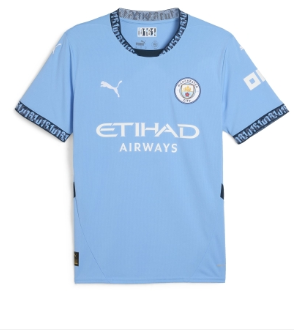
\includegraphics[height=0.1\textwidth]{img_maillots/img1.png}\\
    \st{80,00 \euro}\\
    -20\%

    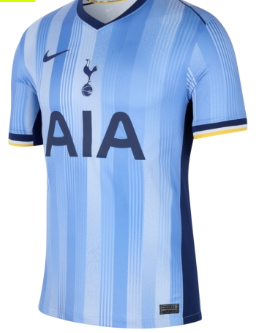
\includegraphics[height=0.1\textwidth]{img_maillots/img2.png}\\
    \st{70,00 \euro}\\
    -15\%

    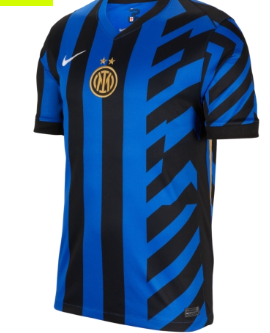
\includegraphics[height=0.1\textwidth]{img_maillots/img3.png}\\
    \st{90,00 \euro}\\
    -34\%
    \end{multicols}
    \end{center}
\end{exo}

\prof{
    Pour la correction, penser à faire un schéma dans chacun des cas.
}

\begin{exo}[Avec calulatrice][]
    
    Ce graphique représente l'évolution de la démographie en Seine-Saint-Denis (source : Wikipedia).
\begin{center}
    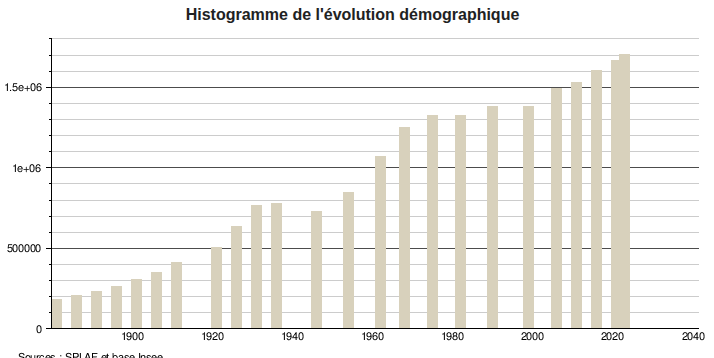
\includegraphics[width=0.5\textwidth]{population_saint_denis.png}
\end{center}

\begin{enumerate}
    \item Combien y avait-il d'habitants en 1980 ? En 2023 ?
    \item En déduire l'évolution de la population entre 1980 et 2023, en pourcentage.
\end{enumerate}
\end{exo}


\end{multicols}

\end{document}
